\documentclass[a4paper]{article} 
\addtolength{\hoffset}{-2.25cm}
\addtolength{\textwidth}{4.5cm}
\addtolength{\voffset}{-3.25cm}
\addtolength{\textheight}{5cm}
\setlength{\parskip}{0pt}
\setlength{\parindent}{0in}

\usepackage{natbib}
\usepackage{blindtext} % Package to generate dummy text
\usepackage{charter} % Use the Charter font
\usepackage[utf8]{inputenc} % Use UTF-8 encoding
\usepackage{microtype} % Slightly tweak font spacing for aesthetics
\usepackage{amsthm, amsmath, amssymb} % Mathematical typesetting
\usepackage{float} % Improved interface for floating objects
\usepackage{hyperref} % For hyperlinks in the PDF
\usepackage{graphicx, multicol} % Enhanced support for graphics
\usepackage{xcolor} % Driver-independent color extensions
\usepackage{pseudocode} % Environment for specifying algorithms in a natural way
\usepackage[ddmmyyyy]{datetime} % Uses YEAR-MONTH-DAY format for dates
%\usepackage{gensymb}
\usepackage{bibentry}

\usepackage{fancyhdr} % Headers and footers
\pagestyle{fancy} % All pages have headers and footers
\fancyhead{}\renewcommand{\headrulewidth}{0pt} % Blank out the default header
\fancyfoot[L]{} % Custom footer text
\fancyfoot[C]{} % Custom footer text
\fancyfoot[R]{\thepage} % Custom footer text
\newcommand{\note}[1]{\marginpar{\scriptsize \textcolor{red}{#1}}} % Enables comments in red on margin

%----------------------------------------------------------------------------------------

\usepackage{adjustbox}
\usepackage{float}
\usepackage{multicol}
\usepackage{pgfplots, pgfplotstable}
%-------------------------------
%	TITLE VARIABLES (identify your work!)
%-------------------------------

\newcommand{\yourname}{Jakob Kralj 4.A} % replace YOURNAME with your name
\newcommand{\papertitle}{Prosti pad} % replace X with paper title

\begin{document}

%-------------------------------
%	TITLE SECTION (do not modify unless you really need to)
%-------------------------------
\fancyhead[C]{}
\hrule \medskip
\begin{minipage}{0.295\textwidth} 
\raggedright
\footnotesize
\yourname \hfill\\ 
\end{minipage}
\begin{minipage}{0.69\textwidth} 
\centering 
\Large
\text{\papertitle}\\ 
\normalsize 
\end{minipage}
\medskip\hrule 
\bigskip


%-------------------------------
%	ASSIGNMENT CONTENT (add your responses)
%-------------------------------

\section*{Naloga:} % this is an example

Ugotovi, kako se pri prostem padu s časom spreminja hitrost telesa. Iz strmine grafa $v(t)$ določi vrednost težnega pospeška.

\section*{Potrebščine:}

ŠMI, žici, brnač, trak, utež.

\section*{Skica:}
\begin{center}
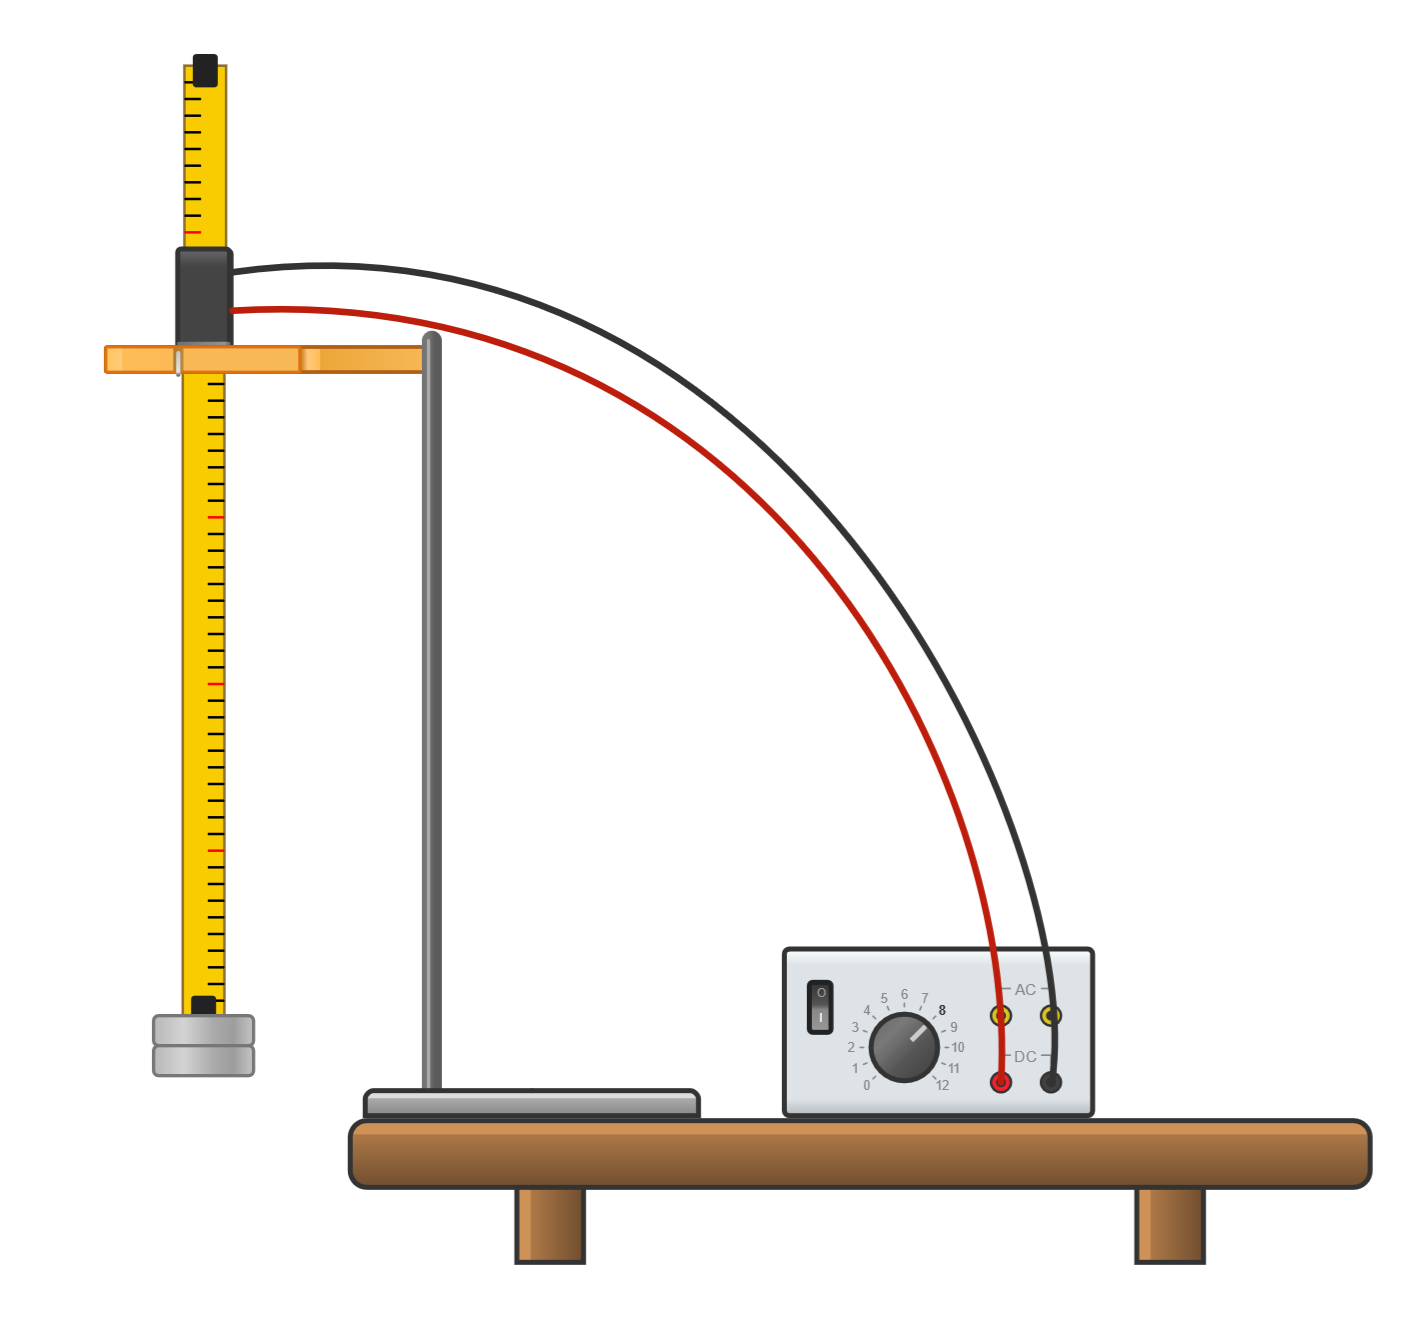
\includegraphics[scale=0.3]{skica.png}
\end{center}
\section*{Meritve:}

Trak z utežjo spusti skozi brnač. Frekvenca peresa brnača je 50Hz. Na traku dobiš odtise peresa brnača, iz katerih razbereš, kako se je s časom spreminjala pot padajoče uteži. Iz traku odčitaj 10 meritev. Vrednosti za čas in pot zapiši v tabelo.


\begin{table}[H]
   \centering
\begin{tabular}{lll}
   $t[s]$ & $s[m]$ & $v[\frac{m}{s}]$ \\
0,02 & 0,006  & 0,3   \\
0,04 & 0,015  & 0,375 \\
0,06 & 0,0275 & 0,458 \\
0,08 & 0,0425 & 0,531 \\
0,10  & 0,0605 & 0,605 \\
0,12 & 0,0825 & 0,688 \\
0,14 & 0,1075 & 0,768 \\
0,16 & 0,135  & 0,844 \\
0,18 & 0,166  & 0,922 \\
0,20  & 0,1995 & 0,998
\end{tabular}
\end{table}



\section*{Rezultati in obdelava podatkov:}

\pgfplotstableread{
X Y
0.02	0.3
0.04	0.375
0.06	0.458
0.08	0.531
0.1	0.605
0.12	0.688
0.14	0.768
0.16	0.844
0.18	0.922
0.2	0.998
}\datatable

\begin{center}
\begin{tikzpicture}
\begin{axis}[
   legend pos= north west,
   title = {$v(t)$},
   xlabel={Čas $[s]$},
   ylabel={Hitrost $[\frac{m}{s}]$}
   ]
\addplot [only marks, mark = *] table {\datatable};
\addplot [thick, red] table[
    y={create col/linear regression={y=Y}}
] % compute a linear regression from the input table
{\datatable};
\addlegendentry{$m(V)$}
\addlegendentry{%
$\pgfmathprintnumber{\pgfplotstableregressiona} \cdot x
\pgfmathprintnumber[print sign]{\pgfplotstableregressionb}$}
\end{axis}
\end{tikzpicture}
\end{center}

Strmina grafa je enaka pospešku, ki znaša $3.89 \frac{m}{s^2}$

Te rezultate lahko nanesemo tudi na graf $s(t)$:
\pgfplotstableread{
X Y
0.02	0.006
0.04	0.015
0.06	0.0275
0.08	0.0425
0.1	0.0605
0.12	0.0825
0.14	0.1075
0.16	0.135
0.18	0.166
0.2	0.1995
}\datatable

\begin{center}
\begin{tikzpicture}
\begin{axis}[
   legend pos= north west,
   title = {$s(t)$},
   xlabel={Čas $[s]$},
   ylabel={Razdalja $[m]$},
   ]
\addplot [only marks, mark = *] table {\datatable};
\end{axis}
\end{tikzpicture}
\end{center}

Graf sledi obliki polinoma druge stopnje. 

\section*{Interpretacija}
Dobljena vrednost močno odstopa od pričakovane vrednosti.
V osnovi je to posledica trenja med brnačem in trakom, zračnega upora in nenatančnega merjenja. Za večjo natančno bi bilo potrebno najti način merjenja razdalje brez trenja, kot je recimo laserski meter in ta eksperiment opraviti v vakuumu. 

\end{document}